% Options for packages loaded elsewhere
\PassOptionsToPackage{unicode}{hyperref}
\PassOptionsToPackage{hyphens}{url}
%
\documentclass[
]{article}
\usepackage{amsmath,amssymb}
\usepackage{lmodern}
\usepackage{iftex}
\ifPDFTeX
  \usepackage[T1]{fontenc}
  \usepackage[utf8]{inputenc}
  \usepackage{textcomp} % provide euro and other symbols
\else % if luatex or xetex
  \usepackage{unicode-math}
  \defaultfontfeatures{Scale=MatchLowercase}
  \defaultfontfeatures[\rmfamily]{Ligatures=TeX,Scale=1}
\fi
% Use upquote if available, for straight quotes in verbatim environments
\IfFileExists{upquote.sty}{\usepackage{upquote}}{}
\IfFileExists{microtype.sty}{% use microtype if available
  \usepackage[]{microtype}
  \UseMicrotypeSet[protrusion]{basicmath} % disable protrusion for tt fonts
}{}
\makeatletter
\@ifundefined{KOMAClassName}{% if non-KOMA class
  \IfFileExists{parskip.sty}{%
    \usepackage{parskip}
  }{% else
    \setlength{\parindent}{0pt}
    \setlength{\parskip}{6pt plus 2pt minus 1pt}}
}{% if KOMA class
  \KOMAoptions{parskip=half}}
\makeatother
\usepackage{xcolor}
\usepackage[margin=1in]{geometry}
\usepackage{graphicx}
\makeatletter
\def\maxwidth{\ifdim\Gin@nat@width>\linewidth\linewidth\else\Gin@nat@width\fi}
\def\maxheight{\ifdim\Gin@nat@height>\textheight\textheight\else\Gin@nat@height\fi}
\makeatother
% Scale images if necessary, so that they will not overflow the page
% margins by default, and it is still possible to overwrite the defaults
% using explicit options in \includegraphics[width, height, ...]{}
\setkeys{Gin}{width=\maxwidth,height=\maxheight,keepaspectratio}
% Set default figure placement to htbp
\makeatletter
\def\fps@figure{htbp}
\makeatother
\setlength{\emergencystretch}{3em} % prevent overfull lines
\providecommand{\tightlist}{%
  \setlength{\itemsep}{0pt}\setlength{\parskip}{0pt}}
\setcounter{secnumdepth}{5}
\usepackage{booktabs}
\usepackage{longtable}
\usepackage{array}
\usepackage{multirow}
\usepackage{wrapfig}
\usepackage{float}
\usepackage{colortbl}
\usepackage{pdflscape}
\usepackage{tabu}
\usepackage{threeparttable}
\usepackage{threeparttablex}
\usepackage[normalem]{ulem}
\usepackage{makecell}
\usepackage{xcolor}
\ifLuaTeX
  \usepackage{selnolig}  % disable illegal ligatures
\fi
\usepackage[]{natbib}
\bibliographystyle{plainnat}
\IfFileExists{bookmark.sty}{\usepackage{bookmark}}{\usepackage{hyperref}}
\IfFileExists{xurl.sty}{\usepackage{xurl}}{} % add URL line breaks if available
\urlstyle{same} % disable monospaced font for URLs
\hypersetup{
  pdftitle={Phantom-Words with simultaneous visual presentation - Results},
  pdfkeywords={Keywords},
  hidelinks,
  pdfcreator={LaTeX via pandoc}}

\title{Phantom-Words with simultaneous visual presentation - Results}
\author{Ansgar D. Endress\\
City, University of London}
\date{}

\begin{document}
\maketitle
\begin{abstract}
Abstract (to be written)
\end{abstract}

\hypertarget{predictions}{%
\section{Predictions}\label{predictions}}

The predictions for the current experiment were unclear. On the one
hand, it is plausible that observers might encode entire scenes when
they are presented simultaneously. If so, they should not accept
phantom-words. On the other hand, statistical learning might operate
similarly for simultaneous as for sequential presentation. If so, the
results with sequential presentations should be replicated, especially
because the shapes appear as distinct individual shapes rather than
wholes. Further, presenting the shapes as whole in an object (i.e., in
the white on black presentation) might encourage observers to process
the combination of shapes as a single hole, leading to the rejection of
phantom words.

REMOVED INTERACTION TERM IN GLMM

MAKE SEPARATE TABLES FOR GLMMS

\hypertarget{analysis}{%
\section{Analysis}\label{analysis}}

\hypertarget{demographics}{%
\subsection{Demographics}\label{demographics}}

In the current population, about a third of the sample usually needs to
be excluded from analysis due to insufficient attention. Unfortunately,
the present experiment does not offer a clear performance-based
criterion, as participants might genuinely be unable to perform the
task. However, as we are mainly interested in the performance on trials
involving phantom-words, and rely on the earlier literature to show that
participants can learn statistical relations \emph{in principle}, we
exclude those participants not exceeding an accuracy of 50\% on word
vs.~part-word trials. This criterion led to the removal of 23 and 53
participants from the students and testable samples, respectively.

The demographics of the remaining participants is given in Table
\ref{tab:vsl-simultaneous-fa-demographics}; age and gender were not
recorded due to experimenter error.

\begin{table}

\caption{\label{tab:vsl-simultaneous-fa-demographics}Demograpics for Experiment 1. Age and gender have not been recorded due to experimenter error}
\centering
\begin{tabular}[t]{llr}
\toprule
color.type & subjectGroup & N\\
\midrule
\addlinespace[0.3em]
\multicolumn{3}{l}{\textbf{testable}}\\
\hspace{1em}black.on.white & 11 & 7\\
\hspace{1em}black.on.white & 12 & 4\\
\hspace{1em}black.on.white & 13 & 7\\
\hspace{1em}black.on.white & 14 & 7\\
\hspace{1em}black.on.white & 15 & 5\\
\hspace{1em}black.on.white & 16 & \vphantom{1} 2\\
\hspace{1em}black.on.white & 17 & 7\\
\hspace{1em}black.on.white & 18 & 5\\
\hspace{1em}black.on.white & 19 & 3\\
\hspace{1em}black.on.white & 20 & 4\\
\hspace{1em}black.on.white & TOTAL & 51\\
\hspace{1em}white.on.black & 1 & 3\\
\hspace{1em}white.on.black & 10 & 5\\
\hspace{1em}white.on.black & 2 & 7\\
\hspace{1em}white.on.black & 3 & 6\\
\hspace{1em}white.on.black & 4 & 6\\
\hspace{1em}white.on.black & 5 & 3\\
\hspace{1em}white.on.black & 6 & 6\\
\hspace{1em}white.on.black & 7 & 5\\
\hspace{1em}white.on.black & 8 & 7\\
\hspace{1em}white.on.black & 9 & 9\\
\hspace{1em}white.on.black & TOTAL & 57\\
\addlinespace[0.3em]
\multicolumn{3}{l}{\textbf{students}}\\
\hspace{1em}black.on.white & 11 & 2\\
\hspace{1em}black.on.white & 12 & 3\\
\hspace{1em}black.on.white & 13 & 2\\
\hspace{1em}black.on.white & 14 & 2\\
\hspace{1em}black.on.white & 15 & 1\\
\hspace{1em}black.on.white & 16 & 2\\
\hspace{1em}black.on.white & 19 & 2\\
\hspace{1em}black.on.white & 20 & 1\\
\hspace{1em}black.on.white & TOTAL & 15\\
\hspace{1em}white.on.black & 10 & 1\\
\hspace{1em}white.on.black & 2 & 1\\
\hspace{1em}white.on.black & 3 & 3\\
\hspace{1em}white.on.black & 5 & 2\\
\hspace{1em}white.on.black & 7 & 2\\
\hspace{1em}white.on.black & 8 & 1\\
\hspace{1em}white.on.black & 9 & 2\\
\hspace{1em}white.on.black & TOTAL & 12\\
\bottomrule
\end{tabular}
\end{table}

\hypertarget{analysis-by-accuracy}{%
\subsection{Analysis by accuracy}\label{analysis-by-accuracy}}

In the analyses, below we will ask three sets of questions.

\begin{enumerate}
\def\labelenumi{\arabic{enumi}.}
\tightlist
\item
  Do participants learn? We compare accuracy and difference scores in
  all cells to their respective baselines.
\item
  Is it harder to discriminate between words and phantom-words than
  between words and part-words?

  \begin{itemize}
  \tightlist
  \item
    Difference score
  \item
    One-way ANOVA
  \end{itemize}
\item
  Is it harder to reject part-words with respect to words compared to
  phantom-words?

  \begin{itemize}
  \tightlist
  \item
    Difference score
  \item
    One-way ANOVA
  \end{itemize}
\item
  Do any of these effects interact with color.type?
\end{enumerate}

\begin{table}

\caption{\label{tab:vsl-simultaneous-fa-descriptives}Descriptives in the naming experiment. *d* represent difference scores.}
\centering
\begin{tabular}[t]{lrrrr}
\toprule
 & *N* & *M* & *SE* & *p.wilcoxon*\\
\midrule
\addlinespace[0.3em]
\multicolumn{5}{l}{\textbf{testable - black.on.white}}\\
\hspace{1em}w.pw & 51 & 69.118 & 1.496 & 0.000\\
\hspace{1em}w.phw & 51 & 49.346 & 2.012 & 0.985\\
\hspace{1em}phw.pw & 51 & 63.562 & 2.516 & 0.000\\
\hspace{1em}d.relative.w.pw.w.phw & 51 & 0.178 & 0.021 & 0.000\\
\hspace{1em}d.relative.w.pw.ph.pw & 51 & 0.056 & 0.021 & 0.026\\
\hspace{1em}d.absolute.w.pw.w.phw & 51 & 19.771 & 2.309 & 0.000\\
\hspace{1em}d.absolute.w.pw.ph.pw & 51 & 5.556 & 2.568 & 0.037\\
\addlinespace[0.3em]
\multicolumn{5}{l}{\textbf{students - black.on.white}}\\
\hspace{1em}w.pw & 15 & 66.667 & 2.381 & 0.001\\
\hspace{1em}w.phw & 15 & 50.556 & 5.355 & 0.875\\
\hspace{1em}phw.pw & 15 & 60.556 & 1.968 & 0.002\\
\hspace{1em}d.relative.w.pw.w.phw & 15 & 0.165 & 0.058 & 0.018\\
\hspace{1em}d.relative.w.pw.ph.pw & 15 & 0.047 & 0.029 & 0.143\\
\hspace{1em}d.absolute.w.pw.w.phw & 15 & 16.111 & 5.980 & 0.018\\
\hspace{1em}d.absolute.w.pw.ph.pw & 15 & 6.111 & 3.714 & 0.111\\
\addlinespace[0.3em]
\multicolumn{5}{l}{\textbf{testable - white.on.black}}\\
\hspace{1em}w.pw & 57 & 69.152 & 1.395 & 0.000\\
\hspace{1em}w.phw & 57 & 49.269 & 2.065 & 0.905\\
\hspace{1em}phw.pw & 57 & 58.626 & 1.985 & 0.000\\
\hspace{1em}d.relative.w.pw.w.phw & 57 & 0.182 & 0.021 & 0.000\\
\hspace{1em}d.relative.w.pw.ph.pw & 57 & 0.091 & 0.021 & 0.000\\
\hspace{1em}d.absolute.w.pw.w.phw & 57 & 19.883 & 2.332 & 0.000\\
\hspace{1em}d.absolute.w.pw.ph.pw & 57 & 10.526 & 2.521 & 0.001\\
\addlinespace[0.3em]
\multicolumn{5}{l}{\textbf{students - white.on.black}}\\
\hspace{1em}w.pw & 12 & 67.361 & 2.262 & 0.002\\
\hspace{1em}w.phw & 12 & 52.778 & 5.392 & 0.623\\
\hspace{1em}phw.pw & 12 & 47.917 & 4.167 & 0.765\\
\hspace{1em}d.relative.w.pw.w.phw & 12 & 0.141 & 0.051 & 0.019\\
\hspace{1em}d.relative.w.pw.ph.pw & 12 & 0.180 & 0.045 & 0.004\\
\hspace{1em}d.absolute.w.pw.w.phw & 12 & 14.583 & 5.580 & 0.041\\
\hspace{1em}d.absolute.w.pw.ph.pw & 12 & 19.444 & 4.831 & 0.006\\
\bottomrule
\end{tabular}
\end{table}

\begin{table}

\caption{\label{tab:vsl-simultaneous-fa-sw}Shapiro-Wilk test results for the different cells.}
\centering
\begin{tabular}[t]{lrrl}
\toprule
test.type & W & p.value & p<=.05\\
\midrule
\addlinespace[0.3em]
\multicolumn{4}{l}{\textbf{testable - black.on.white}}\\
\hspace{1em}w.pw & 0.855 & 0.000 & ***\\
\hspace{1em}w.phw & 0.946 & 0.021 & *\\
\hspace{1em}phw.pw & 0.971 & 0.251 & \\
\hspace{1em}d.relative.w.pw.w.phw & 0.979 & 0.512 & \\
\hspace{1em}d.relative.w.pw.ph.pw & 0.965 & 0.135 & \\
\hspace{1em}d.absolute.w.pw.w.phw & 0.967 & 0.168 & \\
\hspace{1em}d.absolute.w.pw.ph.pw & 0.967 & 0.159 & \\
\addlinespace[0.3em]
\multicolumn{4}{l}{\textbf{students - black.on.white}}\\
\hspace{1em}w.pw & 0.826 & 0.008 & **\\
\hspace{1em}w.phw & 0.979 & 0.963 & \\
\hspace{1em}phw.pw & 0.888 & 0.063 & .\\
\hspace{1em}d.relative.w.pw.w.phw & 0.939 & 0.365 & \\
\hspace{1em}d.relative.w.pw.ph.pw & 0.913 & 0.151 & \\
\hspace{1em}d.absolute.w.pw.w.phw & 0.924 & 0.221 & \\
\hspace{1em}d.absolute.w.pw.ph.pw & 0.910 & 0.136 & \\
\addlinespace[0.3em]
\multicolumn{4}{l}{\textbf{testable - white.on.black}}\\
\hspace{1em}w.pw & 0.854 & 0.000 & ***\\
\hspace{1em}w.phw & 0.952 & 0.025 & *\\
\hspace{1em}phw.pw & 0.966 & 0.114 & \\
\hspace{1em}d.relative.w.pw.w.phw & 0.979 & 0.405 & \\
\hspace{1em}d.relative.w.pw.ph.pw & 0.884 & 0.000 & ***\\
\hspace{1em}d.absolute.w.pw.w.phw & 0.956 & 0.035 & *\\
\hspace{1em}d.absolute.w.pw.ph.pw & 0.894 & 0.000 & ***\\
\addlinespace[0.3em]
\multicolumn{4}{l}{\textbf{students - white.on.black}}\\
\hspace{1em}w.pw & 0.865 & 0.056 & .\\
\hspace{1em}w.phw & 0.926 & 0.338 & \\
\hspace{1em}phw.pw & 0.952 & 0.663 & \\
\hspace{1em}d.relative.w.pw.w.phw & 0.972 & 0.933 & \\
\hspace{1em}d.relative.w.pw.ph.pw & 0.914 & 0.237 & \\
\hspace{1em}d.absolute.w.pw.w.phw & 0.948 & 0.603 & \\
\hspace{1em}d.absolute.w.pw.ph.pw & 0.872 & 0.069 & .\\
\bottomrule
\end{tabular}
\end{table}

\begin{center}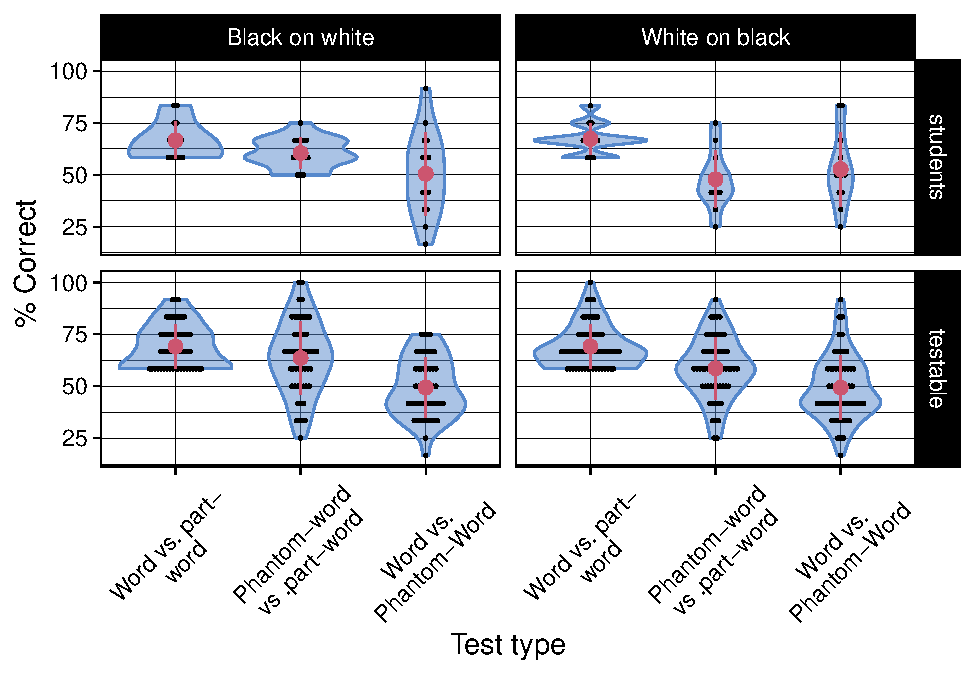
\includegraphics[width=0.8\linewidth]{vsl_phamtoms_simultaneous_results_files/figure-latex/vsl-simultaneous-fa-plot-accuracy-1} \end{center}

\begin{table}[!h]

\caption{\label{tab:vsl-simultaneous-fa-aov}ANOVA for accuracy scores in the naming experiment}
\centering
\resizebox{\linewidth}{!}{
\begin{tabular}[t]{lrrrrrrlr}
\toprule
Effect & DFn & DFd & SSn & SSd & F & p & p<.05 & ges\\
\midrule
\addlinespace[0.3em]
\multicolumn{9}{l}{\textbf{students - Black on white - Word vs. Part-Words vs. Phantom-Words vs. Part-Words}}\\
\hspace{1em}test.type & 1 & 14 & 2.80e+02 & 1352 & 2.901 & 0.111 &  & 0.130\\
\addlinespace[0.3em]
\multicolumn{9}{l}{\textbf{testable - Black on white - Word vs. Part-Words vs. Phantom-Words vs. Part-Words}}\\
\hspace{1em}test.type & 1 & 50 & 7.87e+02 & 8241 & 4.775 & 0.034 & * & 0.035\\
\addlinespace[0.3em]
\multicolumn{9}{l}{\textbf{students - Black on white - Word vs. Part-Words vs. Words vs. Phantom-Words}}\\
\hspace{1em}test.type & 1 & 14 & 1.95e+03 & 3505 & 7.777 & 0.014 & * & 0.224\\
\addlinespace[0.3em]
\multicolumn{9}{l}{\textbf{testable - Black on white - Word vs. Part-Words vs. Words vs. Phantom-Words}}\\
\hspace{1em}test.type & 1 & 50 & 9.97e+03 & 6664 & 74.791 & 0.000 & * & 0.388\\
\addlinespace[0.3em]
\multicolumn{9}{l}{\textbf{students - White on black - Word vs. Part-Words vs. Phantom-Words vs. Part-Words}}\\
\hspace{1em}test.type & 1 & 11 & 2.27e+03 & 1412 & 17.672 & 0.001 & * & 0.455\\
\addlinespace[0.3em]
\multicolumn{9}{l}{\textbf{testable - White on black - Word vs. Part-Words vs. Phantom-Words vs. Part-Words}}\\
\hspace{1em}test.type & 1 & 56 & 3.16e+03 & 9967 & 17.743 & 0.000 & * & 0.146\\
\addlinespace[0.3em]
\multicolumn{9}{l}{\textbf{students - White on black - Word vs. Part-Words vs. Words vs. Phantom-Words}}\\
\hspace{1em}test.type & 1 & 11 & 1.28e+03 & 1884 & 7.452 & 0.020 & * & 0.236\\
\addlinespace[0.3em]
\multicolumn{9}{l}{\textbf{testable - White on black - Word vs. Part-Words vs. Words vs. Phantom-Words}}\\
\hspace{1em}test.type & 1 & 56 & 1.13e+04 & 8525 & 74.016 & 0.000 & * & 0.366\\
\addlinespace[0.3em]
\multicolumn{9}{l}{\textbf{students - Both - Word vs. Part-Words vs. Phantom-Words vs. Part-Words}}\\
\hspace{1em}color.type & 1 & 25 & 4.76e+02 & 1826 & 6.510 & 0.017 & * & 0.094\\
\hspace{1em}test.type & 1 & 25 & 2.18e+03 & 2764 & 19.691 & 0.000 & * & 0.322\\
\hspace{1em}color.type:test.type & 1 & 25 & 5.93e+02 & 2764 & 5.360 & 0.029 & * & 0.114\\
\addlinespace[0.3em]
\multicolumn{9}{l}{\textbf{testable - Both - Word vs. Part-Words vs. Phantom-Words vs. Part-Words}}\\
\hspace{1em}color.type & 1 & 106 & 3.23e+02 & 21679 & 1.581 & 0.211 &  & 0.008\\
\hspace{1em}test.type & 1 & 106 & 3.48e+03 & 18208 & 20.263 & 0.000 & * & 0.080\\
\hspace{1em}color.type:test.type & 1 & 106 & 3.33e+02 & 18208 & 1.936 & 0.167 &  & 0.008\\
\addlinespace[0.3em]
\multicolumn{9}{l}{\textbf{students - Both - Word vs. Part-Words vs. Words vs. Phantom-Words}}\\
\hspace{1em}color.type & 1 & 25 & 2.84e+01 & 5481 & 0.129 & 0.722 &  & 0.003\\
\hspace{1em}test.type & 1 & 25 & 3.14e+03 & 5388 & 14.571 & 0.001 & * & 0.224\\
\hspace{1em}color.type:test.type & 1 & 25 & 7.78e+00 & 5388 & 0.036 & 0.851 &  & 0.001\\
\addlinespace[0.3em]
\multicolumn{9}{l}{\textbf{testable - Both - Word vs. Part-Words vs. Words vs. Phantom-Words}}\\
\hspace{1em}color.type & 1 & 106 & 2.50e-02 & 20004 & 0.000 & 0.991 &  & 0.000\\
\hspace{1em}test.type & 1 & 106 & 2.12e+04 & 15189 & 147.693 & 0.000 & * & 0.376\\
\hspace{1em}color.type:test.type & 1 & 106 & 1.68e-01 & 15189 & 0.001 & 0.973 &  & 0.000\\
\bottomrule
\end{tabular}}
\end{table}

\begin{table}[!h]

\caption{\label{tab:vsl-simultaneous-fa-plot-glmer-correct-calculate}Binary mixed model results}
\centering
\resizebox{\linewidth}{!}{
\begin{tabular}[t]{lrrlrrlrr}
\toprule
\multicolumn{1}{c}{ } & \multicolumn{3}{c}{Log-odds} & \multicolumn{3}{c}{Odd ratios} & \multicolumn{2}{c}{ } \\
\cmidrule(l{3pt}r{3pt}){2-4} \cmidrule(l{3pt}r{3pt}){5-7}
term & Estimate & SE & CI & Estimate & SE & CI & t & p\\
\midrule
\addlinespace[0.3em]
\multicolumn{9}{l}{\textbf{testable - Black on white - Word vs. Part-Words vs. Phantom-Words vs. Part-Words}}\\
\hspace{1em}test.typew.pw & 0.254 & 0.122 & {}[0.0138, 0.493] & 1.289 & 0.158 & {}[1.01, 1.64] & 2.073 & 0.038\\
\addlinespace[0.3em]
\multicolumn{9}{l}{\textbf{students - Black on white - Word vs. Part-Words vs. Phantom-Words vs. Part-Words}}\\
\hspace{1em}test.typew.pw & 0.264 & 0.220 & {}[-0.166, 0.695] & 1.303 & 0.286 & {}[0.847, 2] & 1.204 & \vphantom{1} 0.229\\
\addlinespace[0.3em]
\multicolumn{9}{l}{\textbf{testable - Black on white - Word vs. Part-Words vs. Words vs. Phantom-Words}}\\
\hspace{1em}test.typew.pw & 0.832 & 0.119 & {}[0.598, 1.07] & 2.297 & 0.274 & {}[1.82, 2.9] & 6.982 & \vphantom{1} 0.000\\
\addlinespace[0.3em]
\multicolumn{9}{l}{\textbf{students - Black on white - Word vs. Part-Words vs. Words vs. Phantom-Words}}\\
\hspace{1em}test.typew.pw & 0.674 & 0.218 & {}[0.246, 1.1] & 1.961 & 0.428 & {}[1.28, 3.01] & 3.089 & 0.002\\
\addlinespace[0.3em]
\multicolumn{9}{l}{\textbf{testable - White on black - Word vs. Part-Words vs. Phantom-Words vs. Part-Words}}\\
\hspace{1em}test.typew.pw & 0.459 & 0.113 & {}[0.236, 0.681] & 1.582 & 0.180 & {}[1.27, 1.98] & 4.042 & 0.000\\
\addlinespace[0.3em]
\multicolumn{9}{l}{\textbf{students - White on black - Word vs. Part-Words vs. Phantom-Words vs. Part-Words}}\\
\hspace{1em}test.typew.pw & 0.808 & 0.244 & {}[0.33, 1.29] & 2.243 & 0.547 & {}[1.39, 3.62] & 3.315 & 0.001\\
\addlinespace[0.3em]
\multicolumn{9}{l}{\textbf{testable - White on black - Word vs. Part-Words vs. Words vs. Phantom-Words}}\\
\hspace{1em}test.typew.pw & 0.836 & 0.113 & {}[0.616, 1.06] & 2.308 & 0.260 & {}[1.85, 2.88] & 7.422 & 0.000\\
\addlinespace[0.3em]
\multicolumn{9}{l}{\textbf{students - White on black - Word vs. Part-Words vs. Words vs. Phantom-Words}}\\
\hspace{1em}test.typew.pw & 0.613 & 0.244 & {}[0.135, 1.09] & 1.847 & 0.450 & {}[1.15, 2.98] & 2.516 & 0.012\\
\addlinespace[0.3em]
\multicolumn{9}{l}{\textbf{testable - Both - Word vs. Part-Words vs. Phantom-Words vs. Part-Words}}\\
\hspace{1em}test.typew.pw & 0.250 & 0.121 & {}[0.0119, 0.488] & 1.284 & 0.156 & {}[1.01, 1.63] & 2.058 & 0.040\\
\hspace{1em}test.typephw.pw:color.typewhite.on.black & -0.209 & 0.117 & {}[-0.437, 0.02] & 0.812 & 0.095 & {}[0.646, 1.02] & -1.788 & 0.074\\
\hspace{1em}test.typew.pw:color.typewhite.on.black & 0.002 & 0.123 & {}[-0.239, 0.242] & 1.002 & 0.123 & {}[0.788, 1.27] & 0.012 & 0.990\\
\addlinespace[0.3em]
\multicolumn{9}{l}{\textbf{students - Both - Word vs. Part-Words vs. Phantom-Words vs. Part-Words}}\\
\hspace{1em}test.typew.pw & 0.264 & 0.220 & {}[-0.166, 0.695] & 1.303 & 0.286 & {}[0.847, 2] & 1.204 & 0.229\\
\hspace{1em}test.typephw.pw:color.typewhite.on.black & -0.512 & 0.226 & {}[-0.955, -0.0691] & 0.599 & 0.135 & {}[0.385, 0.933] & -2.265 & 0.023\\
\hspace{1em}test.typew.pw:color.typewhite.on.black & 0.031 & 0.238 & {}[-0.435, 0.498] & 1.032 & 0.245 & {}[0.647, 1.64] & 0.132 & 0.895\\
\addlinespace[0.3em]
\multicolumn{9}{l}{\textbf{testable - Both - Word vs. Part-Words vs. Words vs. Phantom-Words}}\\
\hspace{1em}test.typew.pw & 0.832 & 0.119 & {}[0.598, 1.07] & 2.297 & 0.274 & {}[1.82, 2.9] & 6.982 & 0.000\\
\hspace{1em}test.typew.phw:color.typewhite.on.black & -0.003 & 0.111 & {}[-0.221, 0.215] & 0.997 & 0.111 & {}[0.802, 1.24] & -0.028 & 0.978\\
\hspace{1em}test.typew.pw:color.typewhite.on.black & 0.002 & 0.120 & {}[-0.234, 0.238] & 1.002 & 0.121 & {}[0.791, 1.27] & 0.013 & 0.989\\
\addlinespace[0.3em]
\multicolumn{9}{l}{\textbf{students - Both - Word vs. Part-Words vs. Words vs. Phantom-Words}}\\
\hspace{1em}test.typew.pw & 0.672 & 0.218 & {}[0.245, 1.1] & 1.958 & 0.426 & {}[1.28, 3] & 3.088 & 0.002\\
\hspace{1em}test.typew.phw:color.typewhite.on.black & 0.089 & 0.226 & {}[-0.354, 0.532] & 1.093 & 0.247 & {}[0.702, 1.7] & 0.394 & 0.693\\
\hspace{1em}test.typew.pw:color.typewhite.on.black & 0.031 & 0.240 & {}[-0.439, 0.502] & 1.032 & 0.248 & {}[0.645, 1.65] & 0.131 & 0.896\\
\bottomrule
\end{tabular}}
\end{table}

\hypertarget{acurracy-by-difference-scores}{%
\subsubsection{Acurracy by difference
scores}\label{acurracy-by-difference-scores}}

\begin{center}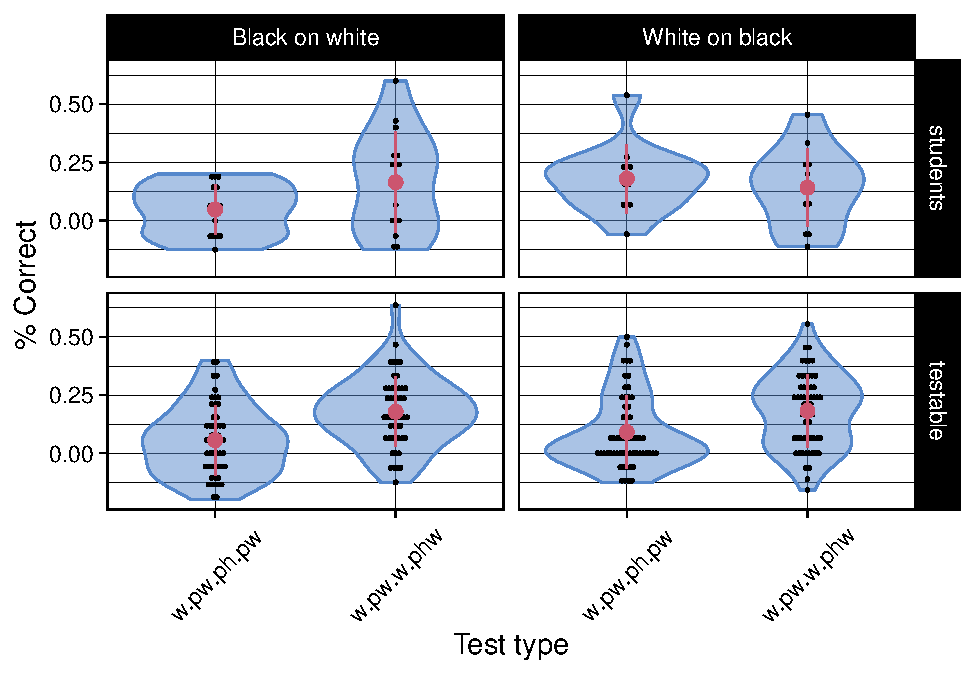
\includegraphics[width=0.8\linewidth]{vsl_phamtoms_simultaneous_results_files/figure-latex/vsl-simultaneous-fa-plot-difference-scores-1} \end{center}

  \bibliography{/Users/endress/ansgar.bib}

\end{document}
